\documentclass[10pt,journal,a4paper]{IEEEtran}
\usepackage[T1]{fontenc}
\usepackage[utf8]{inputenc}
\usepackage{lmodern}
\pdfinfoomitdate=1
\pdftrailerid{}
\pdfsuppressptexinfo=15
\usepackage{amsmath,amssymb,amsthm}
\usepackage{booktabs,array,tabularx}
\usepackage{graphicx}
\usepackage{tikz}
\usetikzlibrary{arrows.meta,positioning}
\usepackage{microtype}
\usepackage{url}
\usepackage[hidelinks]{hyperref}
\usepackage{cite}
\usepackage{etoolbox}
\hypersetup{pdftitle={Conserving Mission Authority Across Delegation and Uncertain Effects},pdfauthor={Mohammed Messaoudene},pdfsubject={Executable research profile, version 0.1.0-research},pdfkeywords={agent authorization, delegation, uncertainty, conformance}}
\newtheorem{proposition}{Proposition}
\newcommand{\code}[1]{\texttt{#1}}
\newcommand{\state}[1]{\ensuremath{\mathsf{#1}}}
\newcommand{\Budget}{\mathbf{B}}
\newcommand{\Free}{\mathbf{F}}
\newcommand{\Pending}{\mathbf{P}}
\newcommand{\Spent}{\mathbf{C}}
\newcommand{\Cost}{\mathbf{q}}
% Generated from evidence/reproduced; do not edit counts by hand.
\newcommand{\UnitCount}{98}
\newcommand{\ProcessCount}{6}
\newcommand{\CaseCount}{10,000}
\newcommand{\StateCount}{1,638}
\newcommand{\TransitionCount}{5,265}
\newcommand{\MutationCount}{4}
\newcommand{\SigMedian}{0.1799}
\newcommand{\SigTail}{0.2985}
\newcommand{\ReserveMedian}{14.0235}
\newcommand{\ReserveTail}{60.212}
\newcommand{\CycleMedian}{54.0588}
\newcommand{\CycleTail}{295.832}

% Release manager may populate these only with actually assigned identifiers.
\newcommand{\SoftwareDOI}{https://doi.org/10.5281/zenodo.22967206}
\newcommand{\PaperDOI}{https://doi.org/10.5281/zenodo.22967208}
\newcommand{\ReleaseRepository}{https://github.com/mohammedmessaoudene-cmd/mission-authority-conservation}

\hyphenation{re-con-cil-i-a-tion crypto-graphic idempo-tency}
\title{Conserving Mission Authority Across\newline Delegation and Uncertain Effects}
\author{Mohammed Messaoudene%
\thanks{M. Messaoudene is a Ma\^itre de conf\'erences B (MCB) at Belhadj Bouchaib University of Ain Temouchent, Ain Temouchent, Algeria (e-mail: \href{mailto:mohammed.messaoudene@univ-temouchent.edu.dz}{mohammed.messaoudene@univ-temouchent.edu.dz}; ORCID: \href{https://orcid.org/0009-0007-4665-2548}{0009-0007-4665-2548}). This affiliation identifies the author's academic appointment only and does not imply sponsorship, collaboration, or endorsement by the university.}}
\markboth{Mission Authority Conservation, Research Report, Version 0.1.0, September 2026}{Messaoudene: Conserving Mission Authority}
\begin{document}
\maketitle
\begin{abstract}
An agent may hold a valid authorization while a delegated mission exceeds its aggregate budget, an approval expires before use, or a lost response causes an already effective action to be retried. These failures concern the composition of authority and execution state rather than the authenticity of a certificate alone. This report specifies an executable research profile that conserves a mission's multidimensional allocation across delegation, reservation, dispatch, and outcome reconciliation. Signed objects bind proposals, resource-derived costs, approvals, permits, and terminal receipts. An unknown outcome retains its reservation; a refund after dispatch requires a durable refusal that excludes later application under the same identifier. A conditional accounting argument is accompanied by a Python/SQLite implementation. The evaluation passes \UnitCount{} test methods, including \ProcessCount{} spawned-process cases, and \CaseCount{} requests from ten authored scenario families. A finite model visits \StateCount{} states and \TransitionCount{} transitions. Four selected source mutations each enable a directly observed unsafe outcome and fail a focused safety test; restoration removes the violation. A conventional transactional baseline provides the same budget and deduplication guarantees on its compared case. Cloning a privileged authority database reproduces 200 units of effects against an initial allocation of 100. The evidence supports a bounded reference profile and conformance corpus, not a new cryptographic primitive, hardware rollback resistance, semantic truth, universal exactly-once execution, or production security.
\end{abstract}
\begin{IEEEkeywords}
agent authorization, bounded delegation, outcome uncertainty, resource budgets, idempotency, conformance testing, failure recovery
\end{IEEEkeywords}

\section{Introduction}
\IEEEPARstart{C}{onsider} a mission that authorizes a total expenditure of 100 units and delegates work to several software agents. Each request can be correctly signed, correctly addressed, and individually below 100 while their combined effects exceed the mission. A second failure occurs when an approval is valid at reservation time but expires before the resource acts. A third occurs when the resource commits an effect and the requester loses its confirmation. Releasing the reservation in that last case does not undo the effect; it creates spending capacity unsupported by the original mission.

These examples separate three questions: who made a request, which action was authorized, and whether that authority remains available at the point of effect. Fine-grained permissions and complete mediation are established subjects of security engineering, not inventions of agent systems~\cite{saltzer1975,rar}. The research problem studied here is their composition with delegated allocations and uncertain execution outcomes. The objective is not to certify that an agent is generally trustworthy. It is to make a small set of effect-level obligations explicit and testable.

We study a \emph{mission authority conservation profile}: a software contract between an authority holder, a deterministic gate, and an effect-producing resource. An agent proposes an invocation. The resource prepares a signed estimate bound to that invocation. The gate reserves the required allocation and releases a narrowly scoped permit only while the relevant authorization remains valid. The resource records either the effect and its receipt, or a terminal refusal. The gate then reconciles its knowledge without treating missing information as proof of non-execution.

\subsection{Research questions}
The study asks whether a compact implementation can preserve componentwise allocation across delegation and concurrent requests (RQ1); bind authorization to the exact action and its temporal conditions (RQ2); preserve uncertainty across a lost reply and process restart without recreating authority (RQ3); and expose its own dependencies through source mutations and adversarial counterexamples (RQ4). A further positioning question asks which observed guarantees also follow from an ordinary, correctly implemented transaction (RQ5).

\subsection{Contributions and boundaries}
The contribution is a reproducible composition, not an originality claim for its constituent mechanisms. It consists of a signed-object profile and action lifecycle; a conditional conservation argument that distinguishes accounting from actual effects; an executable implementation and focused failure corpus; and preserved negative results that delimit its trust assumptions. In particular, the comparison does not establish that a new protocol is indispensable.

The implemented resource produces only SQLite rows representing fictional money, disclosed bytes, or operation counts. There is no payment provider, email service, model inference, hardware enclave, or MCP/A2A binding in this release. Process separation is exercised by a local test fixture, not a production sandbox. The report is a research artifact; it has not undergone independent human peer review or journal acceptance.

\section{Related Work and Positioning}
\subsection{Resource-bounded delegation}
Agent Contracts formalizes multidimensional constraints and conservation rules for hierarchical agent delegation~\cite{agentcontracts}. That work is direct prior art for the use of contracts and non-amplifying child budgets. We do not claim to originate either concept. Our narrower object is the composition of an allocation ledger with action-bound preparation, temporal revalidation, and reconciliation when effect completion is uncertain. We provide failure traces at those boundaries, rather than an empirical comparison against Agent Contracts' implementation or task-quality results.

\subsection{Identity-bound and fine-grained authorization}
OAuth Rich Authorization Requests carries detailed authorization data and assigns interpretation to the authorization and resource servers~\cite{rar}. It is therefore incorrect to describe existing authorization infrastructure as merely encrypted transport. AIP studies verifiable delegation across MCP and A2A~\cite{aip}; aiAuthZ places identity-bound authorization outside the agent host~\cite{aiauthz}. Those approaches are adjacent to the binding and gate roles here. Their papers were used for positioning, not rerun as baselines. The present measurements cannot establish superior attack resistance or lower integration cost.

\subsection{Authority at the effect boundary}
Das's individual Internet-Draft describes bounded release authority, atomic state consumption, rollback resistance, and enforcement where sensitive model information becomes externally usable~\cite{das}. The document is work in progress, not an adopted RFC. Its discussion of recovery leaves ordering, partial failure, expiration, and ambiguous dispatch to a concrete design. Our software profile explores selected aspects of that failure boundary for several fictional effect dimensions. It does not implement the draft's protected hardware or anti-bypass requirements and, in fact, demonstrates failure under privileged state cloning.

\subsection{Earlier artifacts by the author}
AUEC specifies a host-controlled execution contract, including policy narrowing, result semantics, and portable receipts~\cite{auec}. Its cited deterministic profile and pure authorization predicate are not evidence for the consequential-action engine evaluated in this report. Action Outcome Recovery (AOR) preserves an unknown outcome until provider capabilities justify recovery~\cite{aor}. Its recovery principle is inherited here, not rediscovered. The present implementation adds a shared allocation ledger, delegated scopes, and temporal approval checks around that uncertainty. It is a separate laboratory: neither code integration with AUEC/AOR nor inherited protocol conformance is claimed.

\subsection{Transactions, signatures, and attestation}
SQLite supplies local transactional primitives~\cite{sqlatomic,sqlwal}, Ed25519 supplies signatures~\cite{eddsa}, and deterministic encoding makes signed values reproducible. Our encoding accepts a narrower ASCII/integer domain than general JSON Canonicalization Scheme~\cite{jcs}; it is not an implementation of that standard. RATS distinguishes evidence from appraisal and relying-party decisions~\cite{rats}. It provides a vocabulary for a possible stronger execution environment, not proof that this software gate is isolated or honest.

\section{System Model and Requirements}
\subsection{Roles and adversary}
A principal authorizes a root mission. An actor proposes work and may delegate a portion of its allocation. A separate approval role signs action-specific consent where required. A gate serializes authority changes. A resource measures its supported fictional effects, checks permits, and records terminal results. Logical roles have distinct software keys. The original tests host them in one process; additional tests move the resource into a spawned process.

The actor may alter arguments, reuse identifiers, offer another actor's signature, widen a child scope, issue concurrent requests, replay an old permit, or provide a valid-looking request with an invalid approval. The tests also change the clock, resource version, and gate policy at selected boundaries. The adversary cannot forge the pinned signing keys under the assumed signature security. It is not assumed that a signed actor statement is semantically correct.

The positive claims require an honest principal, gate, resource, and policy interpretation; protected signing keys; one non-cloned serialization domain for each root allocation; reliable local transaction behavior; and trustworthy time for expiry decisions. The resource must account for all effects inside the governed path. The implementation does not establish these deployment properties against a privileged host adversary.

\subsection{Authority is not a risk score}
The allocation is a vector $\Budget=(B_0,B_1,B_2)$ of nonnegative integers. Its components represent fictional monetary units, output bytes, and a count of irreversible operations. They are not exchanged or aggregated into a single score. An allowed message with a false statement may pass all three counters. An octet ceiling is not a confidentiality theorem. An authorization signature is not a determination of legal liability.

The principal may issue separate root missions. Consequently, a root allocation is not a global account balance across every mission that the principal could create. Comparing effects against that broader account would require another explicit authority layer, absent from this profile.

\subsection{Required properties}
The gate must reject requests outside the subject, audience, operation, destination, policy, and temporal bounds of their capability chain. Child scopes must be subsets of parent scopes, and child allocations must be removed from the parent's free allocation. The resource must not let repeated presentation of one accepted identifier produce repeated effects. A dispatched or uncertain action must keep its reservation until a corresponding terminal result is reconciled. Revocation must stop new covered dispatches after its local serialization point; it need not recall permits already in flight.

These are conditional safety requirements. Availability is explicitly weaker: lost permits, unavailable receipts, or unresolved uncertainty can immobilize an allocation indefinitely.

\section{Profile and Conservation Argument}
\subsection{Signed objects and exact binding}
An invocation names an identifier, mission, capability, actor, resource audience, operation, destination, parameters, deadline, and policy version. Let $h_a=H(\operatorname{Canon}(a))$ denote its digest. The resource returns a signed preparation containing $h_a$, the cost vector $\Cost$, its version, audience, and expiry. Its digest $h_p$ binds subsequent approvals and permits to the measured proposal.

The gate does not trust an actor-supplied cost. For a payment fixture the resource reads a positive integer amount; for an export it measures one of two fixed byte arrays; for a message it measures the ASCII payload. A version or cost change at application time causes a durable refusal. This behavior establishes consistency for those small fixture operations, not general estimation of future service costs.

An approval binds $h_a$, $h_p$, the capability, revocation generation, expiry, and an affirmative decision. An arbitrary pair of other signatures does not replace the required approval role. The profile requires that role for an export or a fictional payment of at least 50 units. The threshold is a test parameter, not a recommendation for real financial policy.

\begin{table}[t]
\caption{Signed message roles in the executable profile.}
\label{tab:messages}
\centering\small
\begin{tabularx}{\columnwidth}{@{}l l X@{}}
\toprule
Object & Signer & Bound information\\
\midrule
MISSION & Principal & Root scope and allocation\\
DELEGATE & Parent actor & Child subject, scope, allocation\\
INVOKE & Actor & Exact proposed action\\
PREPARED & Resource & Action, cost, resource version\\
APPROVE & Approval role & Action, preparation, epoch, expiry\\
DISPATCH & Gate & Reserved action and validity bound\\
RECEIPT & Resource & Same action and terminal result\\
REVOKE & Principal & Capability and next generation\\
\bottomrule
\end{tabularx}
\end{table}

\subsection{Local and global conservation}
For capability $v$, define allocation $\Budget_v$, free allocation $\Free_v$, pending allocation $\Pending_v$, and locally committed allocation $\Spent_v$. Pending includes reserved, dispatched, and unknown actions. If $\operatorname{ch}(v)$ denotes the direct children, the local accounting rule is
\begin{equation}
\Budget_v=\Free_v+\Pending_v+\Spent_v+
\sum_{u\in\operatorname{ch}(v)}\Budget_u .
\label{eq:local}
\end{equation}
All vector equalities and inequalities are componentwise. Delegation by $\mathbf d$ subtracts $\mathbf d$ from the parent's free allocation and creates a child allocation of that amount. Reserving an action subtracts $\Cost$ from free and adds it to pending. A confirmed effect transfers $\Cost$ from pending to committed. A permitted cancellation transfers it from pending back to free.

\begin{proposition}[Accounting conservation]
For a finite rooted delegation tree, initially satisfying~\eqref{eq:local}, serialized transitions of the specified forms preserve
\begin{equation}
\Budget_r=\sum_{v\in T_r}(\Free_v+\Pending_v+\Spent_v).
\label{eq:global}
\end{equation}
\end{proposition}
\begin{proof}
A reservation, settlement, or cancellation moves the same vector between two terms at one node. A delegation moves a vector from the parent's free allocation to a newly created child's allocation and free term. No other specified transition changes these totals. Summing~\eqref{eq:local} over the tree cancels every non-root allocation once on each side. The root allocation remains, yielding~\eqref{eq:global}. Nonnegative admission checks preserve nonnegativity of all terms.
\end{proof}

The proposition concerns the transition system. It is not a mechanized proof that every Python path refines that system. The code tests and finite exploration supply separate evidence.

\subsection{From accounting to actual effects}
Accounting alone is insufficient. Let $\mathbf E$ be the total cost of effects actually committed at the resource, and let $\mathbf U\leq\sum_v\Pending_v$ be the cost of effects already applied but not yet reconciled by the gate. If each invocation has a resource-enforced unique identity, all its costs are correctly measured, and no refund leaves its permit usable, then
\begin{equation}
\mathbf E=\sum_v\Spent_v+\mathbf U
\ \leq\ \Budget_r .
\label{eq:effects}
\end{equation}
The equality uses the absence of ungoverned effects and dishonest receipts. It fails when a live permit is refunded, an identifier can produce several effects, or the authority domain is cloned. Those failure modes are not repaired by preserving an internally consistent hash chain.

\subsection{Lifecycle and uncertain outcomes}
The gate represents an action by one of five states:
\begin{equation*}
\state{RESERVED},\ \state{DISPATCHED},\ \state{UNKNOWN},
\end{equation*}
\begin{equation*}
\state{COMMITTED},\ \state{ABORTED}.
\end{equation*}
The state \state{UNKNOWN} describes the gate's knowledge, not the resource's physical state. The resource may have committed an effect even though the gate cannot distinguish that outcome from a request that never arrived.

\begin{figure}[t]
\centering
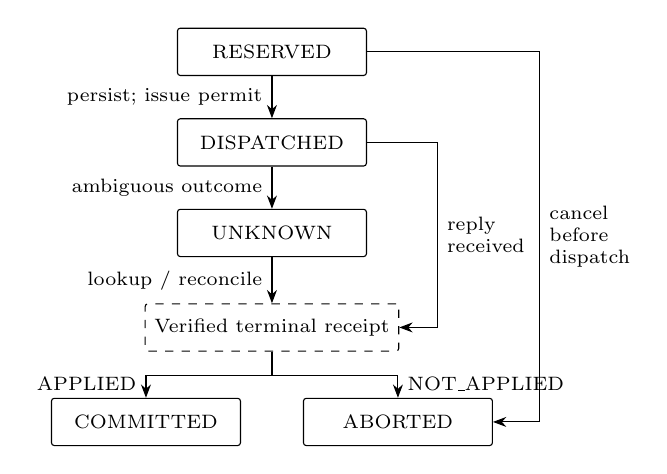
\begin{tikzpicture}[font=\scriptsize,>=Stealth,
box/.style={draw,rounded corners=1pt,minimum width=24mm,minimum height=6mm,align=center}]
\node[box] (r) at (0,0) {RESERVED};
\node[box] (d) at (0,-1.15) {DISPATCHED};
\node[box] (u) at (0,-2.3) {UNKNOWN};
\node[box,dashed,minimum width=32mm] (t) at (0,-3.5) {Verified terminal receipt};
\node[box] (c) at (-1.6,-4.7) {COMMITTED};
\node[box] (a) at (1.6,-4.7) {ABORTED};
\draw[->] (r)--node[left]{persist; issue permit}(d);
\draw[->] (d)--node[left]{ambiguous outcome}(u);
\draw[->] (u)--node[left]{lookup / reconcile}(t);
\draw[->] (d.east) -- (2.1,-1.15) -- node[right,align=left]{reply\\received} (2.1,-3.5) -- (t.east);
\draw[->] (t.south) -- ++(0,-.3) -| node[pos=.7,left]{APPLIED} (c.north);
\draw[->] (t.south) -- ++(0,-.3) -| node[pos=.7,right,align=left]{NOT\_APPLIED} (a.north);
\draw[->] (r.east) -- (3.4,0) -- node[right,align=left]{cancel\\before\\dispatch}(3.4,-4.7) -- (a.east);
\end{tikzpicture}
\caption{Gate lifecycle. The dashed box is a verification step, not an extra action state. After dispatch, a terminal receipt is required for settlement; timeout alone does not refund authority.}
\label{fig:states}
\end{figure}

The resource records an \code{APPLIED} receipt atomically with its fictional effect. A repeated permit returns the existing receipt. A \code{NOT\_APPLIED} receipt is also persisted and bars later application under that identifier. Only this durable refusal supports refund after dispatch. A lookup returning no row provides no such guarantee: a delayed permit may still arrive.

The implementation forbids issuing another permit from \state{DISPATCHED} or \state{UNKNOWN}. A retained permit can be presented again to the resource, which deduplicates it. This is deliberately conservative. If the permit itself disappears before arrival and no terminal receipt can be found, the allocation can remain stranded. A protocol that always resolves this condition would need additional resource-side expiry or cancellation guarantees.

\subsection{Time, policy, and revocation}
The effective permit deadline is
\begin{equation}
t_{\max}=\min(t_a,t_c,t_h),
\label{eq:expiry}
\end{equation}
where $t_a$ is the action deadline, $t_c$ the capability expiry, and $t_h$ the approval expiry when approval is required. Otherwise $t_h$ is omitted. Descendant capability expiry cannot exceed its ancestor's. At dispatch, the gate rechecks the capability chain, its revocation generation, the stored policy version, the resource version, and $t<t_{\max}$. The resource rechecks the permit deadline before applying a new effect.

The gate serializes revocation with dispatch. A permit already issued can still be accepted by an unaware resource before expiry. Therefore the design provides a local stop for new dispatches, not instantaneous global revocation. A globally shared generation is used in this prototype; revoking one capability also invalidates older unstarted reservations in unrelated missions. That conservative behavior costs availability and is not claimed as a desirable production policy.

\section{Implementation and Reproduction Boundary}
\subsection{Storage and execution order}
The reference is implemented in Python. A gate database contains capabilities, remaining allocations, actions, a revocation generation, and a hash-linked event sequence. A separate resource database contains terminal receipts and effect rows. Writes use \code{BEGIN IMMEDIATE}, WAL mode, and \code{synchronous=FULL}. SQLite's guarantees depend on the storage and operating environment~\cite{sqlatomic,sqlwal}; our tests do not validate power-loss behavior of that environment.

The gate persists \state{DISPATCHED} before returning the signed permit. This order prevents a crash from leaving a released permit backed only by an unrecorded reservation. The resource couples its effect and receipt in one local transaction. There is no cross-database transaction. Uncertainty exists precisely between these durable boundaries, and the protocol retains authority while it is unresolved.

Internal gate methods are trusted operations, not authenticated public endpoints. The runtime has no HTTP authentication, TLS channel binding, hardware key storage, or operating-system enforcement that excludes other effect paths. A production API must not expose the laboratory object methods directly.

\subsection{Encoding and cryptographic scope}
Signed envelopes contain a type, key identifier, payload, and lowercase hexadecimal Ed25519 signature. The signed preimage includes a fixed protocol/version prefix, a message-type separator, and the canonical payload/key-identifier pair. The key identifier is the SHA-256 digest of the pinned public key. Public verification needs only the raw public key. No secret keys are published in the evidence.

The codec accepts ASCII strings, bounded integers, booleans, null, lists, and objects, with explicit size and depth bounds. It rejects duplicate keys, floats, non-finite values, and unknown fields where exact object schemas are checked. Monetary values reject booleans even though Python treats booleans as an integer subtype. The encoding is intentionally restricted; full Unicode canonical interoperability is outside this profile. Signatures authenticate objects under pinned keys, not the truth of an estimate or the integrity of the execution host.

\subsection{Spawned-process fixture}
A trusted local pipe fixture starts the resource in a fresh Python process. The child receives an ephemeral resource signing key and the gate's public key. The controller still creates and knows the test keys, and both processes share one host. This exercises a process and persistence boundary without claiming adversarial isolation.

A fault command causes the child to exit with status 73 immediately after the resource transaction returns and before sending a reply. The controller observes end-of-file, marks the action unknown, reopens the gate, starts another resource process, retrieves the persisted receipt, and settles once. Other cases replay a permit after restart, persist an expiry refusal, query a missing receipt, and present the same permit concurrently from two processes.

The fixture initially reset a restarted worker's clock to an earlier test value. The core correctly rejected that rollback. The fixture was corrected to start from the controller's current virtual time and retain it between commands. The failed fixture run is preserved separately; it is not portrayed as a new core vulnerability.

\section{Evaluation Method}
\subsection{Evidence categories and gates}
All experiments use fictional actions. The selected publication run uses Windows, Python 3.11.9, SQLite 3.45.1, and cryptography 46.0.4. The earlier Linux run (Python 3.13.5, SQLite 3.46.1; 89 test methods) remains historical evidence, not the source of the current timing table. The test runner reports the actual number executed, failures, errors, skips, and expected failures. It refuses to emit a positive release result for an empty or partially skipped suite. Experiment conditions use explicit exceptions rather than assertions that Python optimization could remove. Original evidence is not overwritten by a new output run.

The evaluation separates deterministic unit/process cases, generated requests, finite-state exploration, code-level causal controls, and a conventional comparator. None of their counts is interpreted as a statistical estimate of all possible attacks or software reliability. The original 83 tests remain intact; six process-boundary methods and nine evidence-runner regression tests extend them to \UnitCount{}. The nine reporting regressions validate failure detection and evidence retention; they are not nine additional security guarantees.

\subsection{Generated requests}
The request generator uses seed 20260925 and ten authored scenario families. Two families are expected to be accepted and eight rejected. It varies small monetary amounts and tests argument modification, mismatched preparation, wrong mission, missing approval, a wrong signer, and stale policy. Accepted requests are cancelled before dispatch, so this campaign measures admission decisions rather than 10,000 real side effects. Its oracle is authored within the same project and may share its assumptions.

\subsection{Finite-state model}
The model contains three potential actions, each of cost two, against a scalar allocation of four. States encode reservation, dispatch, uncertainty, revocation, resource receipt, and actual effect count. Breadth-first exploration records reachable states and transitions. Safety predicates include nonnegative remaining allocation, conservation, aggregate effect bounds, resource deduplication, and absence of unbacked live permissions. Four intentionally weakened transition systems remove budget admission, refund uncertainty, ignore revocation, or permit duplicate resource effects. The reference must satisfy its finite predicates; each weakened model must produce a counterexample.

This model does not include every Python field, arbitrary delegation depth, parser input, physical clock behavior, or database implementation. There is no proof of refinement from the implementation to the model.

\subsection{Source-level causal controls}
Four selected single-line mutations are applied in disposable source copies. M1 removes the action-budget guard. M2 permits cancellation after dispatch or uncertainty. M3 omits the approval-expiry bound. M4 omits policy revalidation at dispatch. Each control requires one unique source target, a changed hash, an executed target line, a passing baseline test, one focused assertion failure in the mutant without an import/runtime error, a direct unsafe observation, and a passing restoration.

The four experiment workers run concurrently, but they are not independent reviewers or language-model agents. They execute predefined tests against temporary code copies. The original source hash must remain unchanged. This provides sensitivity evidence for four chosen checks, not mutation coverage for the program or an independent security audit.

\subsection{Comparators and negative experiments}
The conventional comparator uses an ordinary SQL transaction and a unique effect identifier. It receives 400 attempts over 200 identifiers against an allocation of 100, with 16 worker threads. The test asks whether it respects its budget and deduplicates requests; it does not implement the whole message profile. It is not penalized for lacking agent-specific terminology.

A privileged-cloning experiment backs up the gate database before consumption, reopens that copy with the same authority keys, and spends from both copies against one resource. This deliberately violates the single-authority assumption. A separate synthetic schedule compares copied per-node limits with disjoint allocations under selected delays; it is not a network measurement or a consensus implementation.

\section{Results}
\subsection{Functional and process evidence}
All \UnitCount{} test methods pass with zero skips and zero expected failures. The original suite includes a 200-request reservation race with 16 threads: exactly 100 unit reservations fit the allocation of 100. Forty presentations of one permit with eight threads produce one resource effect. The six process cases in Table~\ref{tab:process} also pass. Their effects are actual local database rows, but not actual payments or messages.

\begin{table}[t]
\caption{Additional spawned-process cases. Each row is one test method, not a population estimate.}
\label{tab:process}
\centering\small
\begin{tabularx}{\columnwidth}{@{}l X X@{}}
\toprule
ID & Condition & Observed result\\
\midrule
P1 & Normal separate-process call & One effect, one settlement\\
P2 & Exit after commit, before reply & UNKNOWN retained; restart lookup resolves once\\
P3 & Replay after worker restart & Same receipt; no new effect\\
P4 & Approval expires before use & Durable refusal; full refund; replay stays refused\\
P5 & No resource receipt & Allocation remains pending\\
P6 & Two processes, one permit & Same receipt and one effect\\
\bottomrule
\end{tabularx}
\end{table}

The generated campaign returns all \CaseCount{} expected decisions: 2,000 accepted and 8,000 rejected, without oracle disagreements. The finite model visits \StateCount{} states and \TransitionCount{} transitions without a counterexample to its declared predicates. All four weakened model variants produce counterexamples.

\subsection{Direct effects of source mutations}
Each source mutation turns its targeted safety test red, and restoration returns it to green. Table~\ref{tab:mutants} records the direct observations. The M2 trace is particularly instructive: an initial allocation of 1,000 funds a 10-unit permit; refunding that uncertain permit restores 1,000 free units; the still-valid permit produces 10 units, and a subsequent 1,000-unit action raises actual effects to 1,010. A refund transition that looks harmless in an isolated ledger is unsafe when an executable permit remains outside it.

\begin{table*}[t]
\caption{Selected source mutations. Baseline and restored versions pass the focused safety test; each mutant fails it through an assertion, with the changed line executed and a directly observed unsafe outcome.}
\label{tab:mutants}
\centering\small
\begin{tabularx}{\textwidth}{@{}l p{.25\textwidth} X p{.17\textwidth}@{}}
\toprule
ID & Removed or weakened condition & Direct mutant observation & Focused test\\
\midrule
M1 & Remaining action-budget check & An extra unit is reserved after spending 1,000; remaining money becomes $-1$. & No budget overrun\\
M2 & Cancellation restricted to RESERVED & An uncertain live permit is refunded; actual resource effects become 1,010 against 1,000. & UNKNOWN holds budget\\
M3 & Approval bound in permit expiry & At time 1,002 an action is applied although its approval expired at 1,001. & In-flight approval expiry\\
M4 & Stored policy rechecked at dispatch & A permit is issued after the gate changes from the policy used at reservation. & Policy change before dispatch\\
\bottomrule
\end{tabularx}
\end{table*}

\subsection{Conventional baseline and privileged cloning}
The ordinary transactional comparator produces 100 effects and leaves zero free units under its specified concurrent workload. It therefore achieves the same aggregate budget and deduplication objectives on that compared case. This result rules out attributing those properties solely to a new agent protocol. The proposed profile's candidate value is a shared contract and test vocabulary around those mechanisms; adoption benefit was not measured.

In the privileged-cloning experiment, each gate copy authorizes 100 units. The shared resource applies two distinct identifiers for a total of 200. Both gate copies pass their local accounting audit. This does not contradict~\eqref{eq:global}, whose domain is one non-cloned tree, but it invalidates any claim that this artifact protects a global allocation against a malicious operator able to copy its authority state.

\subsection{Local execution cost}
Table~\ref{tab:timing} reports one local run of 300 observations after 20 warm-up iterations. Preparation time is excluded. The end-to-end row covers reservation, permit generation, fictional application, and settlement, without the spawned-process fixture. The percentile is the implementation's empirical order statistic, not a service-level guarantee. Variation in host load and storage behavior is not controlled sufficiently for cross-system ranking.

\begin{table}[t]
\caption{Local elapsed times in milliseconds; one run, software keys and SQLite, not a global revocation benchmark.}
\label{tab:timing}
\centering\small
\begin{tabularx}{\columnwidth}{@{}X r r@{}}
\toprule
Operation & Median & Empirical p99\\
\midrule
Signature verification & \SigMedian & \SigTail\\
Reservation and checks & \ReserveMedian & \ReserveTail\\
Reservation to settlement & \CycleMedian & \CycleTail\\
\bottomrule
\end{tabularx}
\end{table}

\section{Security Analysis and Residual Risk}
\subsection{Identity, meaning, and enforcement}
A valid signature establishes an object's origin relative to a pinned key. It does not establish that its signer is honest, its policy expresses the principal's actual intention, or its payload is true. One retained test authorizes a message containing the fictional false statement \code{2+2=5} to an allowed destination. This is consistent with the contract: the content remains within the admitted operation and byte limit. The system is neither a hallucination detector nor a general defense against malicious instructions inside a valid scope.

An approval key is another explicit limit. The test verifies that the correct role signed the exact action; it does not prove that a human was present, understood the request, or used an uncompromised interface. A production human-approval system would need a separately specified ceremony and evidence for that claim.

\subsection{Revocation and availability}
The gate's local revocation ordering excludes newly dispatched work after the revocation point. It does not exclude a previously issued permit at an unaware resource. Expiry bounds that exposure only under trustworthy clocks and resource checks. The synthetic delay experiment cannot establish a millisecond global revocation bound.

No child-budget reclamation is implemented. Revocation does not erase a child's allocation or cancel its in-flight obligations. Likewise, a permanently missing receipt may leave pending allocation unusable. These choices protect the safety argument by withholding resources rather than guessing that work failed. Their operational cost is real and must be evaluated before deployment.

\subsection{Rollback, logs, and dishonest components}
The clock guard detects movement backward relative to stored time. Restoring both that store and its history defeats the comparison. An event chain can expose inconsistency relative to a retained authentic state, but does not prevent an operator from rewriting or cloning an entire consistent history. The cloned-gate experiment demonstrates this boundary directly.

The resource is also trusted. A signed receipt may be false if its signer is compromised. A cost may omit an ungoverned side channel. A row-level atomic transaction does not make an arbitrary external API action atomic with that row. Reusing this implementation around a real bank transfer or actuator without the provider's terminal-result and deduplication semantics would invalidate the evidence-to-effect argument.

\section{Threats to Validity and Practical Implications}
\subsection{Construct and internal validity}
Test counts measure selected behaviors, not broad security. The generated corpus contains ten authored families; it is not an independent adversarial dataset. The finite model and program were developed within the same workflow, so matching results may reflect shared assumptions. Source mutation gives stronger evidence that four checks matter, but selection of those checks is itself internal. The honest comparator also shares the project's test environment.

The original defects and the later fixture error are retained to avoid presenting a fabricated uninterrupted success history. Publication review also found that three evidence-runner fixes from an earlier local preparation had not been carried into the submitted package: retaining generated mismatch records, counting incomplete ten-case batches, and separating reservation denial from cancellation failure. These fixes and nine reporting regressions were restored before the selected run. The publication pass leaves the original core unchanged and strengthens the surrounding evidence runner and process tests. This makes the delta auditable but does not demonstrate complete defect removal.

\subsection{External and conclusion validity}
No external operator, independently developed engine, or production workload was evaluated. Six local process scenarios do not substitute for multi-host failure injection, packet reordering, Byzantine components, disk failure, or exhaustive crash-point analysis. The use of actual Ed25519 signatures does not certify the key lifecycle. The manuscript's mathematical statements are conditional deductions, not formal verification of the delivered software.

The practical next question is whether a resource integrator can implement the same narrow terminal-result and allocation obligations without depending on this code. A useful adoption result could be shared conformance cases rather than a new transport. The current evidence neither measures integration savings nor establishes market demand or inevitable standardization.

\section{Artifact, Licensing, and Research Practice}
The accompanying artifact contains the reference code, tests, selected historical failures, source mutation diffs and hashes, current execution records, manuscript sources, and a claim--evidence matrix. The original private working archive is identified by its digest but is not redistributed. Raw proposal reports and private correspondence are excluded from the public tree.

To reproduce the selected experiment from the project root:
\begin{verbatim}
python -m pip install -r requirements.txt
python -B run_all.py --out local-results
python tools/paper_metrics.py
cd paper
latexmk -pdf main.tex
\end{verbatim}
The default manuscript tables use the archived evidence directory, not an arbitrary later run. A new experiment can be selected explicitly with \code{paper\_metrics.py --evidence}; its environment and source hashes must then remain attached to the new report. Timing and random signing keys vary between runs. Identical scientific expectations, not byte-identical runtime logs, define reproduction. Release archives themselves use deterministic file ordering and fixed ZIP metadata.

The new software, tests, machine-readable schemas, and executable validation materials use Apache-2.0. The paper and narrative specification use CC BY 4.0, with file-level mapping in the artifact. Third-party dependencies retain their own licences and are not relicensed or vendored. No licence change is made to the separately published AUEC or AOR artifacts. ``Contract'' denotes a machine-checkable execution profile here, not a contract of insurance, a legal guarantee, or a transfer of university rights.

\ifdefempty{\SoftwareDOI}{}{Software archive DOI: \expandafter\url\expandafter{\SoftwareDOI}.}
\ifdefempty{\PaperDOI}{}{Report DOI: \expandafter\url\expandafter{\PaperDOI}.}

\section{Conclusion}
A mission's authority must survive more than signature verification. It must remain conserved while agents delegate, requests race, approvals age, and confirmations disappear. The presented profile makes those transitions explicit and tests their composition on an executable resource fixture. The results show sensitivity to four selected source defects and correct behavior in six local process scenarios, while retaining a conventional baseline that is equally safe on its compared objective and a privileged-cloning counterexample that exceeds the original budget.

The supported contribution is a bounded research profile and reproducible failure corpus. Its governing rule is that delegation transfers authority rather than copying it, and uncertainty retains an obligation rather than extinguishing it. Stronger isolation, interoperable bindings, independent implementations, and production utility remain separate claims requiring separate evidence.

\section*{Acknowledgment and AI assistance}
The project was initiated and directed by Mohammed Messaoudene. ChatGPT assisted with research synthesis, reference code, test generation, debugging, experimental execution, manuscript preparation, and artifact packaging. Codex performed the final local reproduction, targeted evidence-runner corrections, reference and claim review, manuscript compilation, and publication preparation. The analytic review roles were performed within the same AI-assisted workflow and do not constitute independent teams or institutional review. The author remains responsible for the report. AI tools are not authors, sponsors, collaborators in the institutional sense, or endorsers.

% Resolved reference list; references.bib is also supplied for journal workflows.
% This file avoids a runtime dependency on BibTeX for the archived report build.
\begin{thebibliography}{13}
\bibitem{saltzer1975} J. H. Saltzer and M. D. Schroeder, ``The protection of information in computer systems,'' \emph{Proceedings of the IEEE}, vol. 63, no. 9, pp. 1278--1308, 1975. doi: 10.1109/PROC.1975.9939.
\bibitem{rar} T. Lodderstedt, J. Richer, and B. Campbell, ``OAuth 2.0 rich authorization requests,'' RFC 9396, May 2023. [Online]. Available: \url{https://www.rfc-editor.org/rfc/rfc9396}
\bibitem{agentcontracts} Q. Ye and J. Tan, ``Agent contracts: A formal framework for resource-bounded autonomous AI systems (full),'' arXiv:2601.08815v3, 25 March 2026. Preprint; the manuscript reports workshop acceptance. [Online]. Available: \url{https://arxiv.org/abs/2601.08815v3}
\bibitem{aip} S. Prakash, ``AIP: Agent identity protocol for verifiable delegation across MCP and A2A,'' arXiv:2603.24775v1, 25 March 2026, preprint. [Online]. Available: \url{https://arxiv.org/abs/2603.24775v1}
\bibitem{aiauthz} S. V. Kodathala, ``aiAuthZ: Off-host, identity-bound authorization for AI agents,'' arXiv:2607.05518v1, 6 July 2026, technical report. [Online]. Available: \url{https://arxiv.org/abs/2607.05518v1}
\bibitem{das} S. Das, ``Beyond attestation: An execution-finality architecture for controlling release and limiting unauthorized extraction and distillation of sensitive frontier AI model information,'' IETF, draft-das-rats-frontier-model-extraction-02, 31 August 2026. Individual Internet-Draft; work in progress, not an adopted RFC. [Online]. Available: \url{https://www.ietf.org/archive/id/draft-das-rats-frontier-model-extraction-02.html}
\bibitem{auec} M. Messaoudene, ``AUEC: A contract layer for verifiable hybrid AI execution,'' technical report, v0.36.0-prestandard, 2026. doi: 10.5281/zenodo.21815335.
\bibitem{aor} M. Messaoudene, ``Action outcome recovery (AOR),'' executable research profile, v0.1.0-research, 2026. doi: 10.5281/zenodo.22866138. [Online]. Available: \url{https://github.com/mohammedmessaoudene-cmd/action-outcome-recovery/tree/v0.1.0-research}
\bibitem{sqlatomic} SQLite Project, ``Atomic commit in SQLite,'' official documentation, accessed 25 September 2026. [Online]. Available: \url{https://sqlite.org/atomiccommit.html}
\bibitem{sqlwal} SQLite Project, ``Write-ahead logging,'' official documentation, accessed 25 September 2026. [Online]. Available: \url{https://sqlite.org/wal.html}
\bibitem{eddsa} S. Josefsson and I. Liusvaara, ``Edwards-curve digital signature algorithm (EdDSA),'' RFC 8032, January 2017. [Online]. Available: \url{https://www.rfc-editor.org/rfc/rfc8032}
\bibitem{jcs} A. Rundgren, B. Jordan, and S. Erdtman, ``JSON canonicalization scheme (JCS),'' RFC 8785, June 2020. [Online]. Available: \url{https://www.rfc-editor.org/rfc/rfc8785}
\bibitem{rats} H. Birkholz, D. Thaler, M. Richardson, N. Smith, and W. Pan, ``Remote ATtestation procedureS (RATS) architecture,'' RFC 9334, January 2023. [Online]. Available: \url{https://www.rfc-editor.org/rfc/rfc9334}
\end{thebibliography}

\end{document}
